
\chapter{ADDITIONAL GENERALIZED COORDINATE NUMBER FIGURES AND SYSTEM IMAGES FOR PLATINUM (321), (112), (765) \& (557)}
\label{app:SI2}


Shown in this appendix are supporting figures for Chapter \ref{chap:facet}.
Additional GCN plots as well as system figures are displayed below.
\newpage



The step-wandering all of the surfaces exhibit during the simulation can hinder
an easy interpretation of the generalized coordination figures. Figure
\ref{fig:557GCN} provides an additional ideal surface to complement the (321)
figure shown in Chapter \ref{chap:facet}. The roughness of the (557) surface is
less than that of the (321) surface which is indicated by the fewer number of GCN
peaks. 

\begin{figure}
\centering
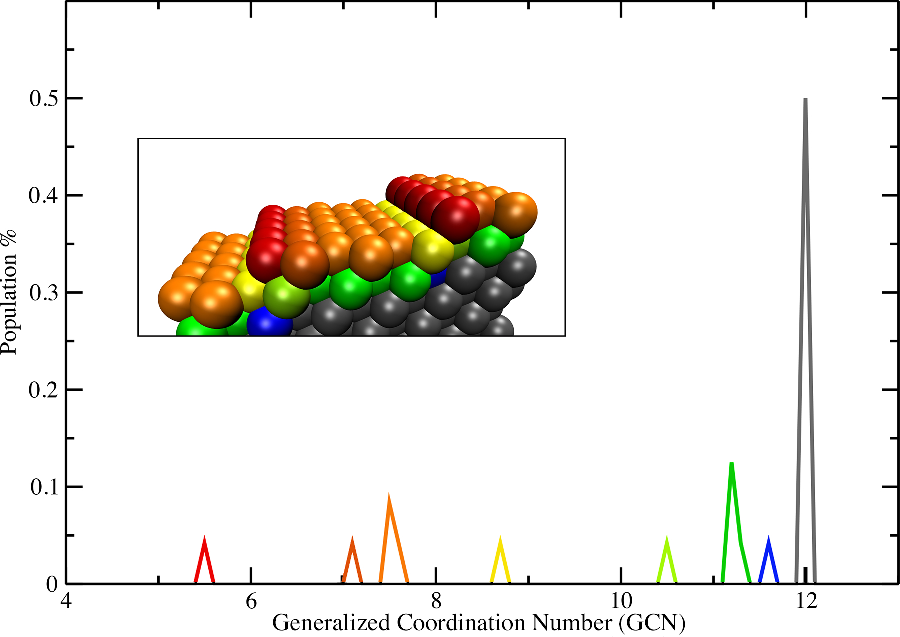
\includegraphics[width=0.9\linewidth]{../figures/appB/557_ideal_gcn.pdf}
\caption{A graph of the generalized coordination number of an ideal Pt (557)
system colored to match the inset figure. Other than the bulk (GCN=12), the
(557) surface displays three primarily different surface sites, the edge atoms
(red, GCN=5.5), the plateaus (orange, GCN=7.2,7.5) and the slightly eclipsed
atoms beneath the step (yellow, GCN=8.7). Subsurface atoms have a larger GCN
than the surface atoms, but are still less than the bulk GCN of 12.}
\label{fig:557GCN}
\end{figure}
\newpage


As the \ce{Pt} (557) did not undergo step doubling in these simulations, the
generalized coordination numbers describing the system were not expected to
largely change, as seen in Figure \ref{fig:557lsGCN}.

\begin{figure}
\centering
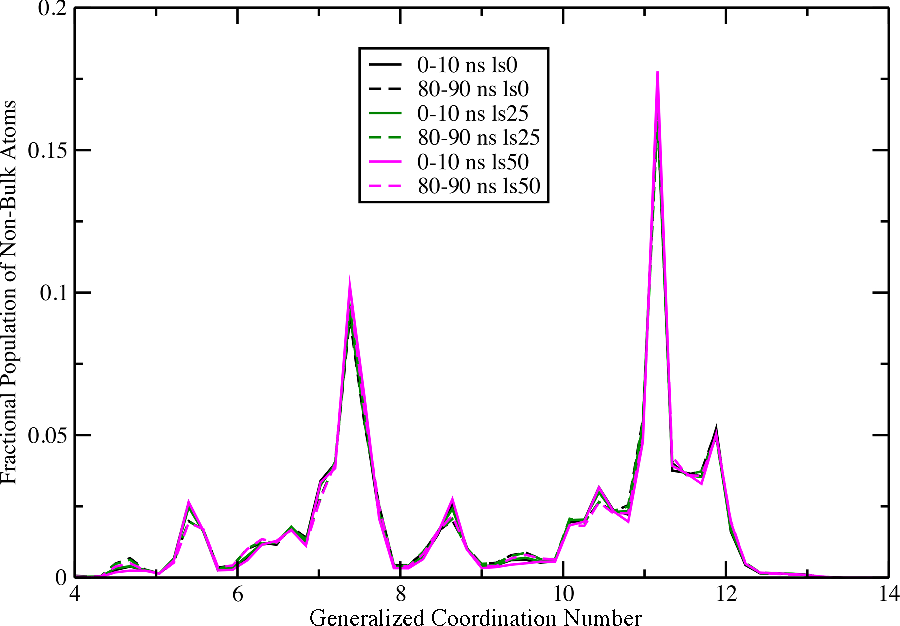
\includegraphics[width=0.9\linewidth]{../figures/appB/557ls_GCNF.pdf}
\caption{Plots of the average GCN for the non-bulk atoms of the \ce{Pt} (557)
LS systems. Solid lines represent the averaged GCN during the first 10
nanoseconds of simulation time, while the dotted lines correspond to a time
near the end of the simulations. Black, green and magenta lines depict the 0,
0.25, and 0.5 ML systems respectively. Except for a slight decrease at a GCN of 5.5 and
10.5, minimal changes were observed.}
\label{fig:557lsGCN}
\end{figure}
\newpage


The slight increase in the peak at GCN=7.5 suggests that this measurement is
sensitive to minor surface reconstructions, like the step-edge doubling and
disappearance highlighted in Figure \ref{fig:765Edge}. Beyond the
reconstruction on the MS 0.5 ML system, very little besides step-wandering was
observed on the (765) surfaces.

\begin{figure}
\centering
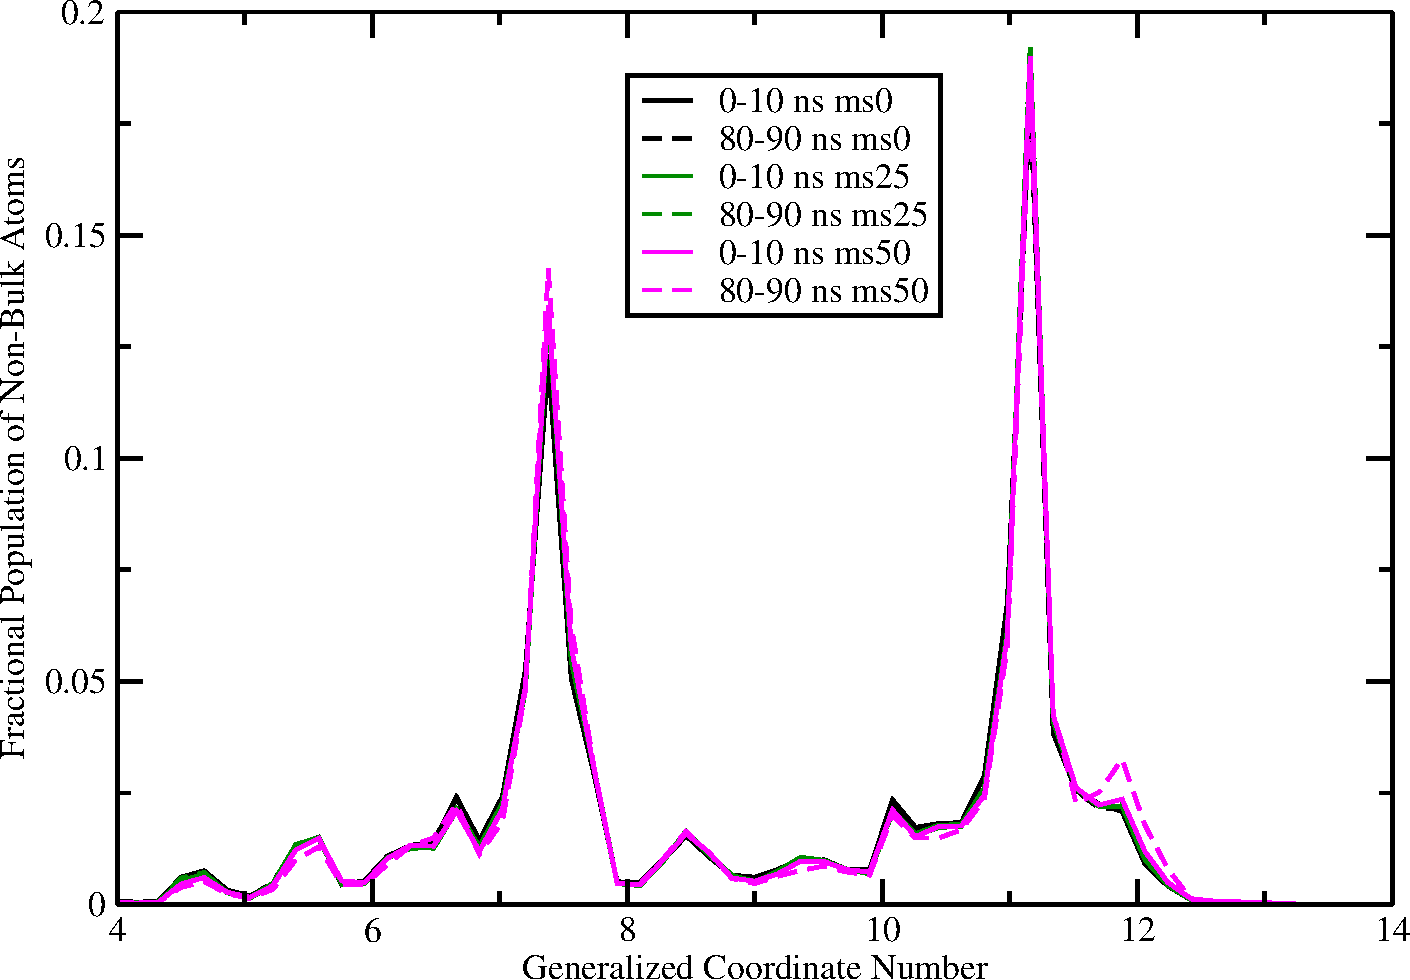
\includegraphics[width=0.9\linewidth]{../figures/appB/765ms_GCNF.pdf}
\caption{Plots of the average GCN for the non-bulk atoms of the \ce{Pt} (765)
MS systems. The slight increases seen at 7.5 and 11.8 capture the
pseudo-doubling process explored in Figure \ref{fig:765Edge}.}
\label{fig:765msGCN}
\end{figure}
\newpage

The increase in the peak at GCN=6.8 for the 0 and 0.5 ML LS systems appears
to be capturing the loss of the clean (765) surface observed on both of these
systems. The 0.25 ML LS system in contrast only exhibited some step-edge
wandering, but generally maintained its displayed edges.

\begin{figure}
\centering
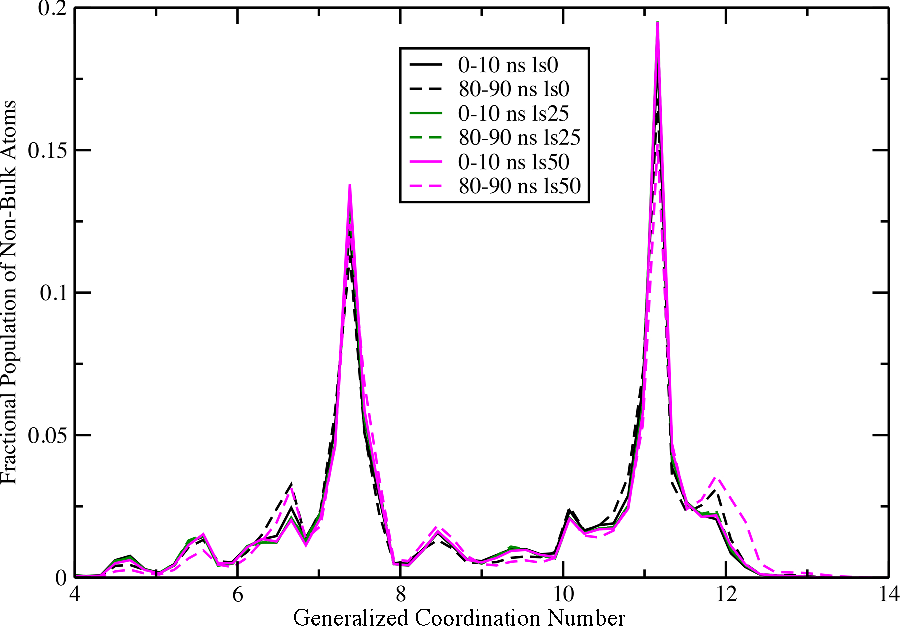
\includegraphics[width=0.9\linewidth]{../figures/appB/765ls_GCNF.pdf}
\caption{Plots of the average GCN for the non-bulk atoms of the \ce{Pt} (765)
LS systems. The slight increases seen at 6.8 and 11.8 for the 0.0 and 0.5 ML
systems appears to capture the disruption seen on these surfaces.}
\label{fig:765lsGCN}
\end{figure}
\newpage

The (112) systems explored in this study suffer from a slight instability at
the temperatures simulated that led to a number of the step-edges sinking
partially into the surface. As highlighted in Figure \ref{fig:112sunken}, a few
of the edges maintained their (100) step facet and were often seen to be a
source for adatom formation. The steps that sunk into the surface on the other hand
rarely ejected adatoms and for the majority of the simulation exhibited
minimal movement on the surface.

\begin{figure}
\centering
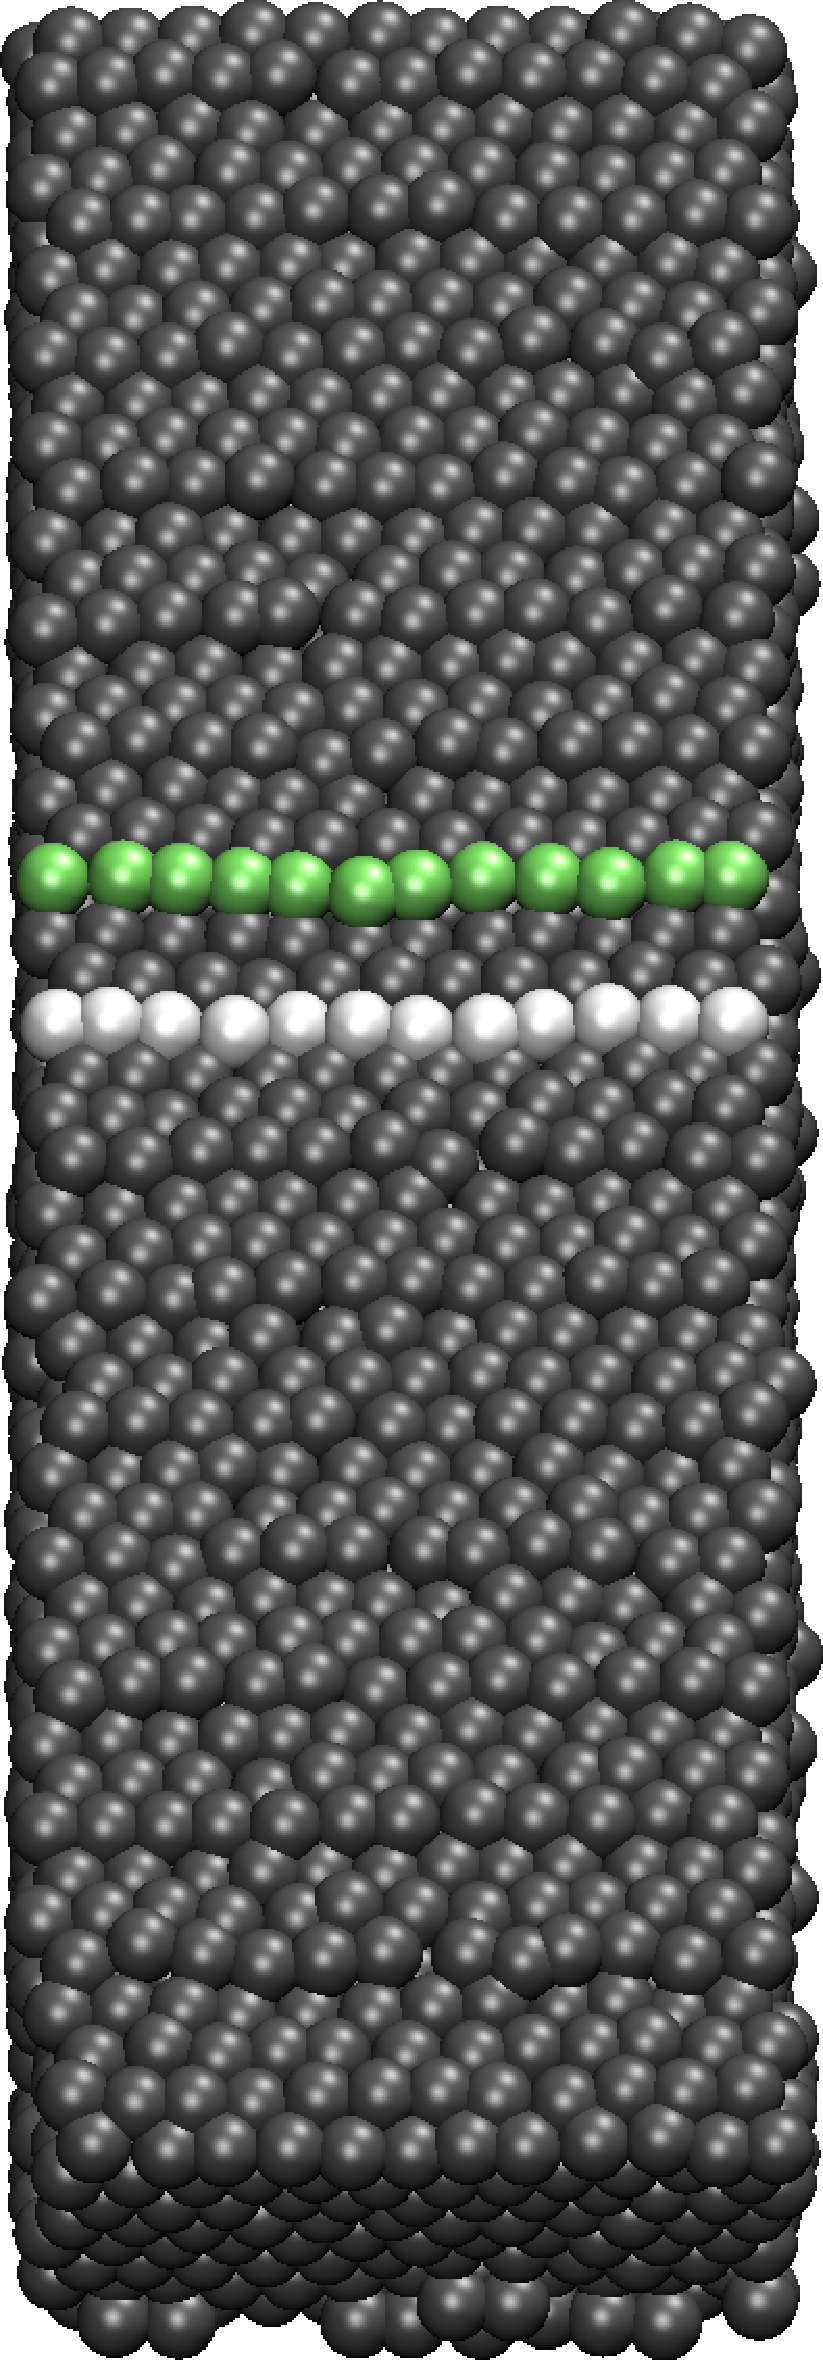
\includegraphics[width=0.3\linewidth]{../figures/appB/112_sunken.pdf}
\caption{The (112) systems, because of their large surface energy, exhibited a
minor refaceting that resulted in many of the (100) steps sinking into
the surface (white) and displaying a (111) sunken edge. A few step edges (lime)
retained their (100) step edge morphology and were the primary source for adatom
formation.}
\label{fig:112sunken}
\end{figure}
\newpage


%\begin{figure}
%\includegraphics[width=0.8\linewidth]{../figures/appB/321MiniDiamonds}
%\caption{The energy required to translocate a kinked atom along the step edge
%is minimal, and on the (321) surfaces this leads to the formation of numerous
%small (111) diamonds on the surface. Systems are shown at (a) the beginning and
%(b)-(c) the end (100 ns) of the simulation for the (112) LS 0.25 ML system.
%While some step-edge doubling is observed, a significant portion of the surface
%has been replaced with these small diamond domains.}
%\label{fig:321Diamonds}
%\end{figure}
%\newpage

The rough edges and large plateaus of the (765) systems were expected to help
distinguish which surface attributes were most important in encouraging or
hindering surface reconstruction. No obvious step-doubling
occurred on these surfaces despite a significant amount of step-wandering
taking place. One event that occurred on the 0.5 ML MS system is displayed in
Figure \ref{fig:765Edge}. What is originally two separate roughened steps, over
the course of the simulation becomes a single step located at an intermediate
distance between the original steps. It appears as if a portion of each step
sinks into the surface leaving the two other sections to meet up to form a
single step edge.

\begin{landscape}
\begin{figure}
\centering
\includegraphics[width=0.9\linewidth]{../figures/appB/765MissingEdge.pdf}
\caption{The (765) MS 0.5 ML system (a) 0 ns, (b) 33.4 ns, (c) 50.2 ns, (d)
75.1 ns, (e) and 100 ns after exposure to CO underwent an unexpected reconstruction.
The identified step-edges in (a), approach each other while also starting
to sink somewhat into the surface. The result in a step-edge that is between
the starting points of either parent, but still of only one atomic height.}
\label{fig:765Edge}
\end{figure}
\end{landscape}
\newpage

